% this file should contain a summary of the propulsion system analysis tools and models including propeller, electric and cycle

% Summary paragraph
The propulsion systems under consideration for NASA's UAM concept vehicles cover a range of different system configurations from all-electric to turbo-electric architectures.
While the various concept vehicles consider different propulsion systems, the systems all contain similar elements leading to the developement of three supporting analysis tools and models.
These tools and models include those for the rotor or propeller, electrical system and gas turbine thermodynamic cycle, which are described in this section.  
For the tiltwing vehicle examined in this study, these three models were combined to form a propulsion system model as shown in Figure \ref{f:turboelectric}. 
In this figure, the gray boxes represent the four rotors/propellers, the red boxes show elements of the electrical system model, and the blue boxes show the components modeled in the thermodynamic cycle.
Each of these three disciplinary models for the propulsion system are described in more detail in the following paragraphs.


\begin{figure}[htb]
\begin{center}
 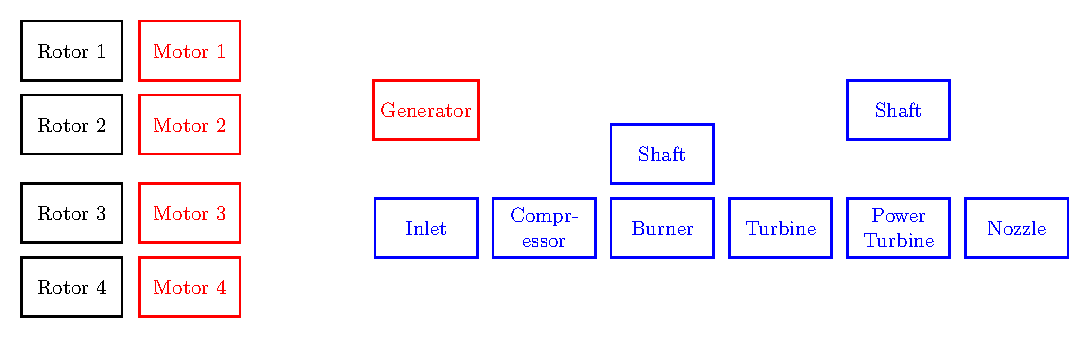
\includegraphics[width=1.0\textwidth]{../Images/Propulsion_system.pdf}
 \caption{Propulsion System Model Components.}
 \label{f:turboelectric}
\end{center}
\end{figure}

\subsubsection{Rotor/Propeller Analysis} %Dan
This section needs a short summary of the propeller analysis in OpenBEMT
\begin{itemize}
    \item Describe the analysis tool and summarize the physics captured by the tool
    \item Describe the inputs and outputs of the code
    \item Make sure to include both design/static information as well as ODE information as appropriate
    \item Reference previous publications on the tool
    \item Describe the model created using the tool for the tiltwing UAM vehicle (include graphic as needed)
\end{itemize}

\subsubsection{Electrical System Analysis} %Eric
To model the electrical components of the propulsion system, a new power systems modeling tool called Zappy was developed on top of the OpenMDAO framework.  
This tool is based on the calculations and methods used in hybrid AC-DC load flow or power flow analysis\cite{hendricks2019load} with additional computational calculations added to capture motor, generator and battery performance. 

In order to used this tool, the user must first define the electrical system layout including the major components and the cables connecting those components.
Additionally, performance information for each of the components in the system must be specified.
This information primarily includes performance maps for the motors and generators (efficiency as a function of shaft speed and torque) as a well as impedances in the cables.
Furthermore, the electrical system takes as input the power demanded by each of the rotors, the power required to operate auxiliary systems, as well as the output voltage provided by the generator.
With this information, the electrical system model can be executed to determine the power that must be produced by the generator as well as the power that is lost to heat in the various components throughout the electrical system.
The analysis of the electrical system is nearly identical between the disciplinary design and mission analysis phases.
The one difference is that during the design phase, the motor and generator maps are scaled to match the design speed, torque and power of those components.  
These computed scalars are then supplied as inputs to the electrical system completed in mission analysis phase. 

The electrical system model for the tiltwing includes the components shown in red in Figure \ref{f:turboelectric}.
The model includes four electric motors, which include an integrated inverter, that are connected to each of the four rotors.
These motor components therefore require DC power which is supplied by an interconnected system of DC cables and electrical buses.
The microgrid produced by this interconnected system was assumed to provided redundancy in the system in the event that failures occurred in one or more lines.
At the other end of the microgrid, a generator along with its integrated rectifier are used to supply DC power to the system.
A battery is also included in the model to supply emergency backup power in the event of failure of the gas turbine engine.
Given this operational assumption, the battery is not charged or discharged during the mission performance modeling.
However, it is sized to provide two minutes of emergency power in the disciplinary design modeling with the battery weight included in the overall mass buildup.


\subsubsection{Thermodynamic Cycle Analysis} %Jeff, Eric
The gas turbine portion of the propulsion system was modeled using a new analysis tool for thermodynamic cycle analysis.
The code, called pyCycle\cite{gray2017chemical,hearn2016optimization}, was selected for this study as it is also built on top of the OpenMDAO framework.
pyCycle differs from other thermodynamic cycle analysis tools such as NPSS in that it provides analytic derivatives to better support gradient-based optimization of the gas turbine as part of larger multidisciplinary optimization studies.


Modeling a gas turbine engine with pyCycle first necessitates that the designer specify the major engine components (i.e. compressor, combustor, turbine, etc.) as well as how these components are connected (both via in terms of flow and shafts).
For each of these components, the user must also provide information about the performance characteristics of the components.
In the disciplinary design phase, this commonly includes information such as the design point component efficiencies, pressure ratios, and performance maps.
In addition, during the design phase the maximum hover power required must be given as an input.
With this information, the gas turbine engine is sized during the design phase with the outputs being the engine mass as well as the flow areas and map scalars which are passed to the model evaluated in the mission analysis phase.
For the mission analysis phase, the same model and connections are evaluated as the design phase with some minor variations in the calculations.  
For this phase, the model again takes in the required shaft power needed by the generator and then determines the fuel flow rate subject to maximum temperature limits.

For the tiltwing turboelectric concept under consideration in this paper, the pyCycle model developed is represented by the blue portion of Figure \ref{f:turboelectric} and is described in more detail in a paper by Chapman.\cite{chapman2018multi}
In summary, the flowpath for the turboshaft engine in this study includes an inlet, compressor, burner, turbine, power turbine and nozzle. 
Furthermore, the compressor and turbine are connected by a shaft with the power turbine connected to the generator by a separate shaft. 
While not included in the simplified graphic of Figure \ref{f:turboelectric}, the model also includes calculations to compute the required turbine cooling flows as well as the effects of small compressor blade heights on compressor efficiency.
For computing the weight of the engine in this study, a simple correlation was developed from historical data for turboshaft engines based on the overall airflow through the engine.
